\newpage
\section{Factory Pattern}
Factory pattern is one of the most used design patterns in Java. This type of design pattern comes under creational pattern as this pattern provides one of the best ways to create an object.
In Factory pattern, we create object without exposing the creation logic to the client and refer to newly created object using a common interface.

\subsection{Class Diagram}

\begin{figure}[h]
\centering
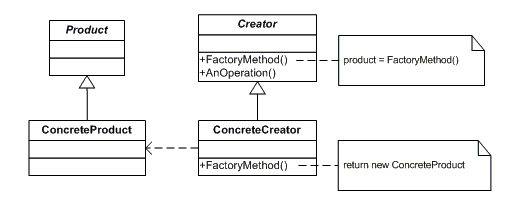
\includegraphics[scale=0.7]{factory}
\caption{Class Diagram of Factory Pattern}
\end{figure}

\newpage
\subsection{Source Code (Java)}

\subsubsection{OS Interface}

\begin{minted}{java}
package factory;

/* OS interface. */

interface OS {
    void spec();
}
\end{minted}

\subsubsection{Android Class}

\begin{minted}{java}
package factory;

package factory;

/* Android class than implements OS interface. */

class Android implements OS {
    public void spec(){
        System.out.println("Most Powerful OS");
    }
}
\end{minted}

\subsubsection{IOS Class}

\begin{minted}{java}
package factory;

/* IOS class than implements OS interface. */

class IOS implements OS {
    public void spec(){
        System.out.println("Most Secure OS");
    }
}
\end{minted}

\subsubsection{Windows Class}

\begin{minted}{java}
package factory;

/* Windows class than implements OS interface. */

class Windows implements OS {
    public void spec(){
        System.out.println("Desktop OS");
    }
}
\end{minted}

\subsubsection{Factory Class - OSFactory}

\begin{minted}{java}
package factory;

class OSFactory {
    public static OS getInstance(String type){
        if (type.equals("ios")){
            return new IOS();
        } else if (type.equals("android")){
            return new Android();
        } else if (type.equals("windows")){
            return new Windows();
        } else {
            return null;
        }
    }
}
\end{minted}

\subsubsection{Driver Class}

\begin{minted}{java}
package factory;

package factory;

/* Driver code for Factory design pattern. */

import java.util.Scanner;

class FactoryDriver {
    public static void main(String[] args) {
        Scanner sc = new Scanner(System.in);
        System.out.print("Enter operating system : ");
        String osType = sc.next();
        
        OS obj = OSFactory.getInstance(osType);
        if(obj != null){
            obj.spec();
        } else {
            System.out.println("Can't create object of given type.");
        }
        sc.close();
    }
}
\end{minted}

\subsection{Output}

\begin{minted}{text}
Enter operating system : android
Most Powerful OS

Enter operating system : ios
Most Secure OS

Enter operating system : windows
Desktop OS

Enter operating system : other
Can't create object of given type.
\end{minted}